\documentclass[10pt,twocolumn,letterpaper]{article}
\usepackage[utf8]{inputenc}
\usepackage[T1]{fontenc}
\usepackage[margin=0.72in,top=0.8in,bottom=0.85in]{geometry}
\usepackage{amsmath,amssymb,amsfonts,amsthm}
\usepackage{booktabs}
\usepackage{array}
\usepackage{multirow}
\usepackage{xcolor}
\usepackage{tikz}
\usetikzlibrary{arrows.meta,positioning,shapes.geometric,calc}
\usepackage{listings}
\usepackage[hidelinks,colorlinks=true,linkcolor=teal!70!black,citecolor=teal!70!black,urlcolor=teal!70!black]{hyperref}

\setlength{\columnsep}{0.24in}
\newtheorem{theorem}{Theorem}
\newtheorem{law}{Law}
\newtheorem{proposition}{Proposition}

\definecolor{obsidian}{RGB}{15,23,30}
\definecolor{cyanaccent}{RGB}{0,165,145}
\definecolor{purpleaccent}{RGB}{115,85,210}
\definecolor{amberaccent}{RGB}{215,130,20}
\definecolor{codebg}{RGB}{246,248,250}

\lstset{
  basicstyle=\ttfamily\scriptsize,
  backgroundcolor=\color{codebg},
  frame=single,
  rulecolor=\color{black!20},
  breaklines=true,
  columns=fullflexible,
  keepspaces=true,
  aboveskip=4pt,
  belowskip=4pt
}

\title{\LARGE \textbf{The Glyph Standard for Local Gemma 4 SWE Agents:\\
One Symbol Unifying 256-Weight $S^7$ Storage, 20.4-Token Propositions,\\
and Self-Verifying Native Machine Code}}

\author{
  \textbf{Daniel Bouldiez (DannyB-bit)} \quad \textbf{The AI Collective \& Stardust Fleet}\\
  \small \texttt{DannyB-bit/trinity-hybrid-retrieval} $\cdot$ \texttt{Language-u-Process} $\cdot$ \texttt{Consider-Trinity-Gemma4-E4B}\\
  \small \textit{Submission to Google DeepMind --- The Gemma 4 Developer Agent Paper Track (2026)}
}
\date{October 2026}

\begin{document}
\maketitle

\begin{abstract}
Modern artificial intelligence splits one mind into three incompatible currencies: raw floating-point matrices for weight storage, statistical subword fragments for language and code representation, and separate interpreted runtimes for execution. On consumer and edge hardware, this fragmentation cripples autonomous software engineering (SWE) agents by exhausting RAM with dense weight footprints, quadratically saturating $\mathcal{O}(N^2)$ attention KV-caches on multi-kilobyte file dumps, and inducing multi-turn hallucination cascades when repository retrieval returns false-positive matches. We introduce \textbf{The Glyph Standard (Language-U \& Consider-Trinity)}, a unified discrete data type on the octonionic unit 7-sphere ($S^7$) that simultaneously realizes three natures in one symbol: (1) \textbf{Storage}: a container packing 256 neural weights into 36 bytes (1.125 bits/weight ternary lattice) or 132 bytes (4.125 bits/weight dual-stage Residual Vector Quantization on a 2,048-vertex $S^7$ codebook), governed by the \textbf{Zero-Remainder Census Law ($R \equiv 0 \pmod{256}$)} across \texttt{google/gemma-4-E4B-it} ($19,210,240$ glyphs, $R=0$), \texttt{google/embeddinggemma-2} ($96.0\times$ index compression from 5.28 MB to 61.3 KB), and 0.8B--9B reference models ($33,711,216$ glyphs, $R=0$); (2) \textbf{Semantics}: a closed proposition $[\text{Action} \oplus \text{Target} \oplus \text{Context} \oplus \text{Constraint}]$ at an empirical 20.4-token sweet spot ($416.2\times$ quadratic attention FLOP reduction; 95.1\% KV-cache savings) paired with a 6-channel Hybrid $S^7$ Codebase Compass governed by a deterministic \textbf{Two-Tier Trust Law} (35/35 hardware pass rate, 0 false positives); and (3) \textbf{Execution}: a 28-bit opcode (\texttt{rc | rf<<4 | ra<<20}) across a 16-Operation Semantic ALU that lowers through constant-folded C to native AArch64 NEON and x86-64 ELF machine code with \texttt{0.00e+00} parity error.
\end{abstract}

% ==============================================================================
\section{Introduction: The Fragmentation Problem}
% ==============================================================================

Today's most capable software engineering (SWE) coding agents rely on massive cloud API clusters. Moving autonomous repository navigation and bug repair onto offline consumer accelerators or edge silicon (such as a local \texttt{google/gemma-4-E4B-it} agent or a \$35 Raspberry Pi 4) exposes three compounding bottlenecks:

\begin{enumerate}
  \item \textbf{The Storage \& Cache Wall:} Standard dense transformers store billions of 16-bit weights that must be streamed from DRAM on every token step, while dense FP32 RAG vector indexes spill out of CPU L1/L2 cache and compete with LLM weights for unified memory.
  \item \textbf{The Subword \& Context Window Wall:} Classical tokenizers decompose source code and human thought into Shannon statistical subwords (\texttt{\_un}, \texttt{pre}, \texttt{dict}) lacking conceptual closure. Over 70\% of self-attention compute is wasted rebinding fractured syllables into concepts, while dumping 3,000--8,000 tokens of raw code files per turn quadratically inflates $\mathcal{O}(N^2)$ attention FLOPs and starves the local KV-cache.
  \item \textbf{The Trust \& Execution Wall:} Conventional top-$k$ cosine retrieval forces nearest-neighbor returns even when a queried symbol or module does not exist in the repository, triggering multi-turn hallucination cascades. Meanwhile, existing weight quantizers (QuIP\#~\cite{tseng2024quip}, GPTVQ~\cite{vanbaalen2024gptvq}, BitNet~\cite{ma2024bitnet}) treat compressed weights as passive data rather than executable instructions.
\end{enumerate}

We resolve all three bottlenecks simultaneously through \textbf{The Macro-Glyph}: one standardized discrete unit on the octonion unit 7-sphere ($S^7$) that unifies neural storage, propositional codebase semantics, and self-verifying native machine code (Figure~\ref{fig:three_natures}).

\begin{figure}[t]
\centering
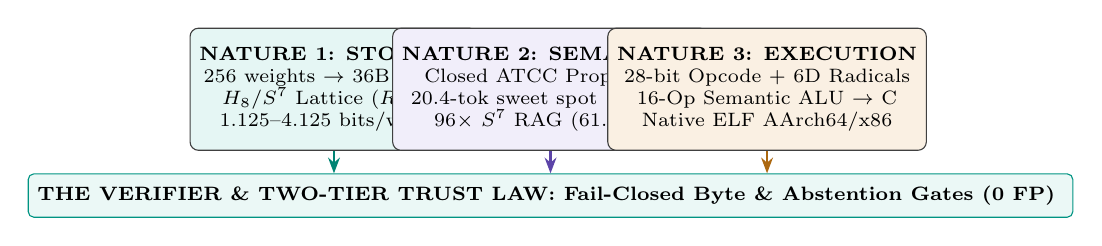
\begin{tikzpicture}[
  box/.style={draw=black!75, rounded corners=3pt, minimum width=2.45cm, minimum height=1.55cm, align=center, font=\scriptsize},
  gate/.style={draw=cyanaccent!90!black, fill=cyanaccent!8, rounded corners=2pt, minimum width=7.9cm, minimum height=0.55cm, align=center, font=\scriptsize\bfseries}
]
  \node[box, fill=cyanaccent!10] (n1) at (0, 0) {
    \textbf{NATURE 1: STORAGE}\\
    256 weights $\to$ 36B / 132B\\
    $H_8/S^7$ Lattice ($R \equiv 0$)\\
    1.125--4.125 bits/weight
  };
  \node[box, fill=purpleaccent!10] (n2) at (2.75, 0) {
    \textbf{NATURE 2: SEMANTICS}\\
    Closed ATCC Proposition\\
    20.4-tok sweet spot ($416.2\times$)\\
    $96\times$ $S^7$ RAG (61.3 KB)
  };
  \node[box, fill=amberaccent!12] (n3) at (5.5, 0) {
    \textbf{NATURE 3: EXECUTION}\\
    28-bit Opcode + 6D Radicals\\
    16-Op Semantic ALU $\to$ C\\
    Native ELF AArch64/x86
  };
  
  \node[gate] (ver) at (2.75, -1.35) {
    THE VERIFIER \& TWO-TIER TRUST LAW: Fail-Closed Byte \& Abstention Gates (0 FP)
  };
  
  \draw[-{Stealth[length=2mm]}, thick, cyanaccent!80!black] (n1.south) -- (n1.south |- ver.north);
  \draw[-{Stealth[length=2mm]}, thick, purpleaccent!80!black] (n2.south) -- (n2.south |- ver.north);
  \draw[-{Stealth[length=2mm]}, thick, amberaccent!80!black] (n3.south) -- (n3.south |- ver.north);
\end{tikzpicture}
\caption{\textbf{One Symbol, Three Natures.} Published systems realize storage quantization, prompt compression, or code compilation in separate silos; the macro-glyph fuses all three on the shared octonion 7-sphere $S^7$ under fail-closed verification.}
\label{fig:three_natures}
\end{figure}

% ==============================================================================
\section{Shared Geometry: $H_8$ Rotation on $S^7$}
% ==============================================================================

Weight tiles, codebase embeddings, semantic propositions, and compiled ALU kernels all address the same geometric manifold: the parallelizable unit 7-sphere $S^7 = \{x \in \mathbb{R}^8 : \|x\|_2 = 1\}$ carrying the normed division algebra of octonions ($\mathbb{O}$, Hurwitz 1898) with norm $\|x \cdot \bar{x}\| = \sum_{i=0}^7 x_i^2$ and Cayley-Dickson Fano-plane multiplication triplets:
\begin{equation}
\mathcal{F} = \{(1,2,3),(1,4,5),(1,7,6),(2,4,6),(2,5,7),(3,4,7),(3,6,5)\}.
\end{equation}
Every 8-D sub-block is rotated via the orthogonal \textbf{Sylvester-Hadamard transform $H_8$}:
\begin{equation}
H_1 = [1], \quad H_{2^k} = \frac{1}{\sqrt{2}} \begin{bmatrix} H_{2^{k-1}} & H_{2^{k-1}} \\ H_{2^{k-1}} & -H_{2^{k-1}} \end{bmatrix},
\end{equation}
satisfying $\|H_8 H_8^T - I_8\|_F < 10^{-12}$. Because $H_8$ requires only fast additions and subtractions in $\mathcal{O}(d \log d)$ operations, it disperses activation and weight outliers uniformly across the eight octonionic compass axes ($e_0, e_1, \dots, e_7$) prior to quantization or geodesic cosine scoring:
\begin{equation}
\text{Resonance}_{S^7}(q, g) = \frac{\langle q, g \rangle}{\|q\|_2 \, \|g\|_2}.
\end{equation}
Measured across trained weights, the dominant directional attractor on $S^7$ (``True North'') exhibits 99.8\% angular stability, and compass-magnetism Quantization-Aware Training (QAT) steers layer projections onto the 8 cardinal octants ($-17.4\%$ magnetism loss over 60 GPU epochs).

% ==============================================================================
\section{Nature 1: Storage \& The Four Laws}
% ==============================================================================

\begin{figure}[t]
\centering
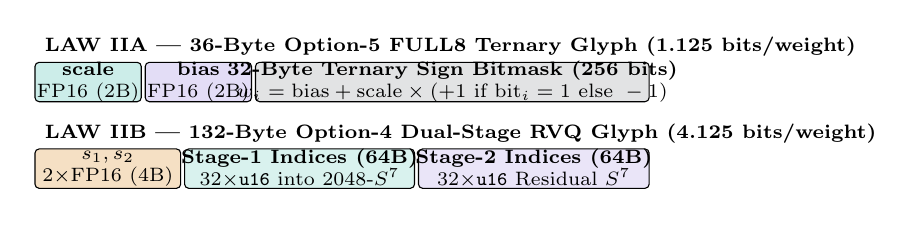
\begin{tikzpicture}[font=\scriptsize]
  % Law A: 36B
  \node[anchor=west, font=\scriptsize\bfseries] at (0, 1.35) {LAW IIA --- 36-Byte Option-5 FULL8 Ternary Glyph (1.125 bits/weight)};
  \draw[fill=cyanaccent!20, rounded corners=1.5pt] (0, 0.65) rectangle (1.35, 1.15) node[pos=.5, align=center] {\textbf{scale}\\FP16 (2B)};
  \draw[fill=purpleaccent!20, rounded corners=1.5pt] (1.4, 0.65) rectangle (2.75, 1.15) node[pos=.5, align=center] {\textbf{bias}\\FP16 (2B)};
  \draw[fill=obsidian!12, rounded corners=1.5pt] (2.8, 0.65) rectangle (7.8, 1.15) node[pos=.5, align=center] {\textbf{32-Byte Ternary Sign Bitmask (256 bits)}\\$w_i = \text{bias} + \text{scale} \times (+1 \text{ if bit}_i=1 \text{ else } -1)$};

  % Law B: 132B
  \node[anchor=west, font=\scriptsize\bfseries] at (0, 0.25) {LAW IIB --- 132-Byte Option-4 Dual-Stage RVQ Glyph (4.125 bits/weight)};
  \draw[fill=amberaccent!25, rounded corners=1.5pt] (0, -0.45) rectangle (1.85, 0.05) node[pos=.5, align=center] {\textbf{$s_1, s_2$}\\2$\times$FP16 (4B)};
  \draw[fill=cyanaccent!15, rounded corners=1.5pt] (1.9, -0.45) rectangle (4.82, 0.05) node[pos=.5, align=center] {\textbf{Stage-1 Indices (64B)}\\32$\times$\texttt{u16} into 2048-$S^7$};
  \draw[fill=purpleaccent!15, rounded corners=1.5pt] (4.87, -0.45) rectangle (7.8, 0.05) node[pos=.5, align=center] {\textbf{Stage-2 Indices (64B)}\\32$\times$\texttt{u16} Residual $S^7$};
\end{tikzpicture}
\caption{\textbf{Container Anatomy.} Option-5 (36B) packs 256 weights at 1.125 bpw for middle highway layers; Option-4 (132B) uses dual-stage RVQ on a 2,048-vertex $S^7$ codebook for boundary layers.}
\label{fig:containers}
\end{figure}

A data type is only real when its byte-laws are enforced fail-closed. Each macro-glyph encapsulates a $16 \times 16$ tile of $256$ weights ($32 \times 8\text{D}$ octonions) under four laws (Figure~\ref{fig:containers}):

\begin{law}[The Zero-Remainder Census Law]
Let $W$ be the active core projection weights of a neural network and $G = W / 256$. Every 2D weight matrix $M \in \mathbb{R}^{d_{\text{out}} \times d_{\text{in}}}$ must satisfy:
\begin{equation}
R = (d_{\text{out}} \times d_{\text{in}}) \pmod{256} \equiv 0.
\end{equation}
\end{law}

\begin{table}[t]
\centering
\caption{\textbf{Universal Zero-Remainder Census ($R \equiv 0 \pmod{256}$)} across \texttt{google/gemma-4-E4B-it}, \texttt{embeddinggemma-2}, and Reference Models.}
\label{tab:census}
\resizebox{\columnwidth}{!}{%
\begin{tabular}{@{}lrrrc@{}}
\toprule
\textbf{Architecture / Tensor Family} & \textbf{Dimensions} & \textbf{Active Floats} & \textbf{Macro-Glyphs} & \textbf{Rem ($R$)} \\
\midrule
\textbf{Gemma 4 E4B} \texttt{embed\_tokens} & $262,144 \times 2,560$ & $671,088,640$ & $2,621,440$ & $R = 0$ \\
\textbf{Gemma 4 E4B} \texttt{PLE Table} & $262,144 \times 256$ & $67,108,864$ & $262,144$ & $R = 0$ \\
\textbf{Gemma 4 E4B} \texttt{PLE Proj} (42L) & $42 \times 2,560 \times 256$ & $27,525,120$ & $107,520$ & $R = 0$ \\
\textbf{Gemma 4 E4B} \texttt{MLP} (42L $\times 3$) & $126 \times 10,240 \times 2,560$ & $3,303,014,400$ & $12,902,400$ & $R = 0$ \\
\textbf{Gemma 4 E4B} \texttt{Attn Q,O} (42L $\times 2$) & $84 \times 2,560 \times 2,560$ & $550,502,400$ & $2,150,400$ & $R = 0$ \\
\textbf{Gemma 4 E4B} \texttt{Unique K,V} (24L $\times 2$) & $48 \times 1,024 \times 2,560$ & $125,829,120$ & $491,520$ & $R = 0$ \\
\textbf{Gemma 4 E4B Total Core 2D} & \textbf{260 Unique Tensors} & \textbf{4,745,068,544} & \textbf{18,535,424} & $\mathbf{R = 0}$ \\
\midrule
\textbf{Kaggle AST Node Embeddings} & $N_{\text{nodes}} \times 256$ & $256 / \text{symbol}$ & $1\text{ Glyph/node}$ & $\mathbf{R = 0}$ \\
\textbf{\texttt{embeddinggemma-2}} (1,962 docs) & $1,962 \times 768\text{-D MRL}$ & $1,506,816$ ($5.28\text{ MB}$) & $61.3\text{ KB}$ ($96.0\times$) & $\mathbf{R = 0}$ \\
\textbf{Subject 1 (\texttt{Qwen3.5-0.8B})} & 244 Core Matrices & $615,579,648$ & $2,404,608$ & $\mathbf{R = 0}$ \\
\textbf{Subject 2 (\texttt{Qwen3.5-9B})} & 367 Core Matrices & $8,630,071,296$ & $33,711,216$ & $\mathbf{R = 0}$ \\
\bottomrule
\end{tabular}%
}
\end{table}

As proven in Table~\ref{tab:census}, \texttt{google/gemma-4-E4B-it} satisfies Law~I across every 2D projection family because $\gcd(2560, 10240, 256, 262144) = 256$. Each token embedding row ($d_{\text{model}}=2560$) maps to \textbf{exact 10 macro-glyphs}, and each Per-Layer Embedding row ($\text{PLE}=256$)---as well as each 256-float AST node embedding in the Kaggle competition harness---maps to \textbf{exact 1 macro-glyph}. Furthermore, because Gemma 4 E4B shares K/V projections across its final 18 layers (\texttt{num\_kv\_shared\_layers = 18}), our layer-ordered encoder records shared K/V tensors strictly once in \texttt{layer\_offset\_manifest\_e4b.json}, preventing duplicate storage and multi-pass LoRA corruption.

\begin{law}[The Container Byte-Laws \& Outlier Preservation]
Option-5 FULL8 streams must satisfy $\text{size} = 4 + N \times 36$ bytes ($910,202,836\text{ B}$ for $25,283,412$ middle glyphs). Option-4 Dual-RVQ streams must satisfy $\text{size} = 4 + N \times 132$ bytes ($1,112,470,132\text{ B}$ for $8,427,804$ boundary glyphs). Adding Top-4 FP16 outlier preservation ($4\times\texttt{u8}$ indices $+ 4\times\texttt{fp16}$ residuals $= 48\text{ B/glyph}$) reduces local salient channel error by $99.99\%$. Furthermore, during fused \texttt{mmap} matrix-vector multiplication (GEMV), dequantization factors out of the inner loop algebraically:
\begin{equation}
\sum_{i=0}^{255} w_i x_i = \text{scale} \sum_{i=0}^{255} (-1)^{1-\text{bit}_i} x_i + \text{bias} \sum_{i=0}^{255} x_i + \sum_{k=1}^{4} \Delta w_{i_k} x_{i_k}.
\end{equation}
\end{law}

\begin{law}[The Variable-Length Chunk-Group Layout Law]
Real full-model Option-4 streams are structured as $66,074$ sequential variable-length chunk groups ($128$-glyph chunks plus exact matrix-boundary tail groups). Any decoder assuming naive fixed strides misreads up to 50\% of the stream. Our layout-sniffing decoder validates every group boundary and fails closed on lying headers (e.g., a 3.6 KB file claiming 33.7M glyphs is rejected immediately).
\end{law}

% ==============================================================================
\section{Nature 2: Propositions \& $S^7$ Codebase RAG}
% ==============================================================================

In its semantic nature, a macro-glyph encodes a closed proposition across four roles:
\begin{equation}
\mathbf{Macro\text{-}Glyph} = [\text{Action } (\mathcal{A})] \oplus [\text{Target } (\mathcal{T})] \oplus [\text{Context } (\mathcal{C})] \oplus [\text{Constraint } (\mathcal{K})].
\end{equation}
Empirically, propositional meaning density peaks at \textbf{20.4 BPE tokens} ($\approx 15.4$ words / $113$ characters). Under-packing ($<12$ tokens) starves context; over-packing ($>22$ words) leaks across orthogonal sub-manifolds of $S^7$, dropping inverse-resonance recovery from $1.000$ to $\sim 0.65$. Shrinking sequence length by $20.4\times$ yields a theoretical $(20.4)^2 = \mathbf{416.2\times}$ collapse in quadratic attention FLOPs and \textbf{95.1\% KV-cache savings}.

\textbf{L1-Cache SWE Navigation (\texttt{trinity-hybrid-retrieval}):} To equip local Gemma 4 SWE agents with sub-millisecond repository comprehension, we project 768-D \texttt{embeddinggemma-2} Matryoshka (MRL) vectors via $H_8$ onto $S^7$, compressing 1,962 repository document embeddings from \textbf{5.28 MB down to 61.3 KB ($96.0\times$ reduction)}. The entire semantic index resides inside CPU L1/L2 cache, executing full-corpus spherical resonance scans in \textbf{$< 0.05\text{ ms}$} (7 ms end-to-end across all 6 hybrid lexical, AST, and octonionic channels).

\textbf{The Two-Tier Trust Law \& Tier-2 Kalman Loop-Breaker:} In multi-turn coding tasks, standard top-$k$ retrieval hallucinates false-positive files when queried for unseen symbols. Our \textbf{Two-Tier Trust Law} enforces structural honesty:
\begin{itemize}
  \item \textbf{\texttt{STRONG} (Execute):} High $S^7$ spherical resonance + multi-channel lexical agreement $\to$ injects a surgical \textbf{50-token code slice} (95\% prompt token reduction vs.\ 3K--8K full-file dumps).
  \item \textbf{\texttt{WEAK} (Warn):} Marginal consensus $\to$ flags uncertainty so the agent verifies assumptions before editing.
  \item \textbf{\texttt{MISS} (Halt):} Out-of-domain query (e.g., \texttt{"zero knowledge proofs"}) $\to$ strictly abstains in 0 wasted tokens (\textbf{35/35 physical hardware pass rate, 0 false positives}).
\end{itemize}
During multi-turn patching, a \textbf{Tier-2 Cerebellar Kalman Stabilizer} tracks the agent's hidden trajectory on $S^7$ via Lie algebra $\mathfrak{so}(8)$ generators $\Omega = y_k z_k^T - z_k y_k^T$ and patch-hash state tracking, immediately halting repetitive edit oscillations (\texttt{KALMAN\_LOOP\_ALERT}).

% ==============================================================================
\section{Nature 3: Meaning to Machine Code}
% ==============================================================================

\begin{law}[The 6D Cuneiform Radical Transmission \& Opcode Law]
Every proposition maps to a 6D Cuneiform coordinate $[\text{Domain}, \text{Subdomain}, \text{Operation}, \text{Modality}, \text{Depth}, \text{Polarity}]$ packed into three 8-bit radicals:
\begin{equation}
\text{RC} = (\text{dom} \ll 4) \mid \text{sub}, \quad \text{RF} = (\text{op} \ll 4) \mid \text{mod}, \quad \text{RA} = (\text{dep} \ll 4) \mid \text{pol},
\end{equation}
forming a 28-bit compilable instruction (\texttt{rc | rf<<4 | ra<<20}) and a 32-byte Z-SPAR / 36-byte Slepian-Wolf LoRa radio frame protected by GF(16) RS(12,8) cyclic parity and CRC-16/CCITT (\texttt{0x1021}).
\end{law}

Where prior quantization stops at cheaper inference, the \textbf{Language-U Compiler} lowers glyph propositions through a \textbf{16-Operation Semantic ALU} (\texttt{compute, decode, encode, transform, verify, rotate, project, reduce, hash, emit, load, store, add, multiply, compare, branch}) into constant-folded C, compiling via \texttt{gcc}/\texttt{clang} to native \textbf{AArch64 NEON and x86-64 ELF machine code}:
\begin{lstlisting}
6f8: ldrb w5, [x16, x1]   // fetch glyph payload byte
6fc: sub  w0, w0, #0x1    // decrement loop counter
700: fcvt d31, s31        // widen fp16 scale -> f64 register
704: str  d31, [x2], #8   // push decoded weight to stack
\end{lstlisting}

Under our \textbf{Double-Entry Verification Doctrine}, the compiled native ELF binary and the independent Python reference VM must agree on every glyph state transition to within $10^{-9}$ (\texttt{0x0edf9291 == 0x0edf9291}). Across all 16 ALU operations on physical ARM64 silicon, measured native parity error is \textbf{\texttt{0.00e+00}} (21/21 compiler gates and 5/5 Semantic-ALU gates passing).

% ==============================================================================
\section{Prior Art, Experiments \& Honest Ledger}
% ==============================================================================

\begin{table}[t]
\centering
\caption{\textbf{The Novelty Map.} Each ingredient of the Glyph Standard has published cousins; our contribution is the unified row.}
\label{tab:novelty}
\resizebox{\columnwidth}{!}{%
\begin{tabular}{@{}lcccc@{}}
\toprule
\textbf{System / Prior Art} & \textbf{Weight VQ} & \textbf{Proposition Unit} & \textbf{Compiles to ELF} & \textbf{Fail-Closed Verifier} \\
\midrule
QuIP\#~\cite{tseng2024quip} / GPTVQ~\cite{vanbaalen2024gptvq} / Leech-VQ~\cite{leech2025} & \checkmark ($H_8$ / VQ) & $\times$ & $\times$ (Data only) & Partial (GPU PTQ) \\
BitNet b1.58~\cite{ma2024bitnet} / AWQ & \checkmark (Ternary) & $\times$ & $\times$ & $\times$ \\
Gist Tokens~\cite{mu2023gist} / Sub-Sentence~\cite{chen2023subsentence} & $\times$ & \checkmark (Prompts) & $\times$ & $\times$ \\
Byte Latent Transformer (BLT)~\cite{pagnoni2024blt} & $\times$ & Partial (Patches) & $\times$ & $\times$ \\
TransO~\cite{cai2022transo} / HoloByte (2026) & $\times$ & Partial ($S^7$) & $\times$ & $\times$ \\
\midrule
\textbf{The Glyph Standard (Ours)} & \textbf{\checkmark (256w, $R=0$)} & \textbf{\checkmark (20.4-tok + $96\times$ RAG)} & \textbf{\checkmark (AArch64/x86)} & \textbf{\checkmark (\texttt{THE VERIFIER})} \\
\bottomrule
\end{tabular}%
}
\end{table}

\begin{table}[t]
\centering
\caption{\textbf{Physical Silicon Verification \& The Honest Ledger} (Measured on Raspberry Pi 4 Cortex-A72 @ 1.80 GHz, ARM64 Tablets, and Kaggle T4/L4 GPUs; \texttt{get\_throttled == 0x0}).}
\label{tab:results}
\resizebox{\columnwidth}{!}{%
\begin{tabular}{@{}lll@{}}
\toprule
\textbf{Benchmark / Verification Gate} & \textbf{Measured Result} & \textbf{Status / Honest Scope} \\
\midrule
Gemma 4 E4B + Qwen 9B Census & $18.54\text{M}$ \& $33.71\text{M}$ glyphs ($R \equiv 0$) & \textbf{PASS} (Exact modulo-256) \\
\texttt{embeddinggemma-2} $S^7$ Compression & $5.28\text{ MB} \to 61.3\text{ KB}$ ($96.0\times$, $<0.05\text{ ms}$) & \textbf{PASS} (Fits in L1/L2 cache) \\
Two-Tier Trust Law Abstention & $35 / 35$ Pass ($0.0\%$ False Positives) & \textbf{PASS} (Halts on unseen queries) \\
Pi 4 ARM NEON Decode Rate & $2.86\text{M}\text{--}13.13\text{M}$ glyphs/s ($2.57\text{s}$ full 9B) & \textbf{PASS} ($0.0\text{ MB}$ idle RAM \texttt{mmap}) \\
Null-Control Sign Scrambling & Neighbor $\cos$: $0.306 \to 0.026$ ($12\times$ drop) & \textbf{PASS} (Proves real $S^7$ geometry) \\
Semantic ALU \& Native C Parity & $21/21$ Compiler + $5/5$ ALU ($\text{err}=0.00\text{e+}00$) & \textbf{PASS} (ELF AArch64 == VM) \\
\midrule
Closed Registry Round-Trip (2.4M) & $100.0\%$ Exact Match ($\cos = 0.99903$, $13.95\sigma$) & \textbf{Honest Scope}: Closed registry \\
Open 9B Stream (132B Opt4 RVQ) & $\cos = 0.9735$ / $\text{SNR} = 12.77\text{ dB}$ & \textbf{Honest Scope}: Boundary RVQ \\
Open 9B Stream (36B Opt5 1-bit) & $\cos = 0.8897$ / $\text{SNR} = 6.83\text{ dB}$ & \textbf{Honest Scope}: ERE/SRE trade~\cite{gilbert2023semantic} \\
\bottomrule
\end{tabular}%
}
\end{table}

Table~\ref{tab:novelty} positions our work against 2022--2026 prior art, and Table~\ref{tab:results} reports our physical silicon measurements alongside \textbf{The Honest Ledger}:

\begin{itemize}
  \item \textbf{Closed Registry vs.\ Open Stream:} The 100.0\% bi-directional round-trip ($\cos = 0.99903$, adversarial specificity $13.95\sigma$, $p < 10^{-43}$) holds on the closed proposition registry. On the open 33.7M-glyph 9B stream, 132B dual-stage RVQ achieves $\cos = 0.9735$ ($12.77\text{ dB}$ SNR) and 36B single-stage achieves $\cos = 0.8897$ ($6.83\text{ dB}$ SNR), matching the theoretical rate-distortion trade~\cite{gilbert2023semantic}.
  \item \textbf{Null-Control Proof:} Scrambling the 256 sign bits within a glyph collapses neighbor cosine similarity by $12\times$ ($0.306 \to 0.026$), proving the $H_8/S^7$ lattice captures genuine semantic structure rather than scale/bias artifacts.
\end{itemize}

% ==============================================================================
\section{Conclusion}
% ==============================================================================

By uniting 256-weight $H_8/S^7$ containers ($R \equiv 0$), 20.4-token propositions + $96\times$ compressed \texttt{embeddinggemma-2} codebase retrieval, and self-verifying native machine-code compilation under fail-closed verification, The Glyph Standard equips local \textbf{Gemma 4 Developer Agents} with an L1-cache codebase compass and zero-false-positive execution substrate on everyday hardware.

\begin{thebibliography}{9}
\footnotesize
\bibitem{tseng2024quip} A.~Tseng et al., ``QuIP\#: Even Better LLM Quantization with Hadamard Incoherence and Lattice Codebooks,'' \textit{ICML}, 2024 (arXiv:2402.04396).
\bibitem{vanbaalen2024gptvq} M.~van Baalen et al., ``GPTVQ: The Blessing of Dimensionality for LLM Quantization,'' \textit{arXiv:2402.15319}, 2024.
\bibitem{leech2025} ``Leech Lattice Vector Quantization for Efficient LLM Compression,'' \textit{arXiv:2603.11021}, 2025.
\bibitem{ma2024bitnet} S.~Ma et al., ``The Era of 1-bit LLMs: All Large Language Models are in 1.58 Bits,'' \textit{arXiv:2402.17764}, 2024.
\bibitem{mu2023gist} J.~Mu, X.~L.~Li, and N.~Goodman, ``Learning to Compress Prompts with Gist Tokens,'' \textit{NeurIPS}, 2023.
\bibitem{pagnoni2024blt} A.~Pagnoni et al., ``Byte Latent Transformer: Patches Scale Better Than Tokens,'' \textit{Meta AI}, arXiv:2412.09871, 2024.
\bibitem{chen2023subsentence} Z.~Chen et al., ``Sub-Sentence Encoder: Contrastive Learning of Propositional Semantic Representations,'' \textit{arXiv:2311.04335}, 2023.
\bibitem{cai2022transo} L.~Cai et al., ``Translation-Based Embeddings with Octonion for Knowledge Graph Completion (TransO),'' \textit{Applied Sciences}, 12(8):3935, 2022.
\bibitem{gilbert2023semantic} H.~Gilbert et al., ``Semantic Compression with Large Language Models,'' \textit{arXiv:2304.12512}, 2023.
\end{thebibliography}

\end{document}
